% \documentclass[table]{beamer}
\documentclass[table,handout]{beamer}
\setbeameroption{show notes}
% \setbeameroption{hide notes}
% \setbeameroption{show only notes}
\usepackage{varwidth}

\newif\ifhide
\newif\ifpost
\newif\ifhideclicker

% \hidetrue
% \hideclickertrue
% \posttrue

\newcommand{\whiteout}[1]{\textcolor{white}{#1}}
% \newcommand{\whiteoutbox}[1]{\fcolorbox{white}{white}{\parbox{\dimexpr \linewidth-2\fboxsep-2\fboxrule}{\whiteout{#1}}}}
% \newcommand{\notebox}[1]{\fcolorbox{blue}{white}{\parbox{\dimexpr \linewidth-2\fboxsep-2\fboxrule}{#1}}}
\newcommand{\whiteoutbox}[1]{\fcolorbox{white}{white}{\parbox{\linewidth}{\whiteout{#1}}}}
\newcommand{\notebox}[1]{\fcolorbox{blue}{white}{\parbox{\linewidth}{#1}}}
\newcommand{\blankbox}[1]{\phantom{\varwidth{\linewidth}\whiteoutbox{#1}\endvarwidth}}
\newcommand{\blank}[1]{\phantom{\varwidth{\linewidth}#1\endvarwidth}}

\ifhide%
    \newcommand{\hmask}[1]{\blank{#1}}%
\else%
    \newcommand{\hmask}[1]{#1}%
\fi

\ifhide%
    \newcommand{\wout}[1]{\whiteout{#1}}%
\else%
    \newcommand{\wout}[1]{#1}%
\fi

\ifhide%
    \newcommand{\hignore}[1]{}%
\else%
    \newcommand{\hignore}[1]{#1}%
\fi

\ifpost%
    \newcommand{\nopost}[1]{}%
\else%
    \newcommand{\nopost}[1]{#1}%
\fi

\ifhideclicker%
    \newcommand{\clickerslide}[1]{\stepcounter{clickerQuestionCounter}%
        \begin{frame}[t]
            \textcolor{blue}{Q \arabic{clickerQuestionCounter}:}
        \end{frame}}
\else%
    \newcommand{\clickerslide}[1]{#1}%
\fi

\ifhide%
    \newcommand{\hidebox}[1]{\blank{#1}}%
\else%
    \newcommand{\hidebox}[1]{\notebox{#1}}%
\fi

\ifhide%
    \newcommand{\wbox}[1]{\whiteoutbox{#1}}%
\else%
    \newcommand{\wbox}[1]{\notebox{#1}}%
\fi

\ifhide%
    \newcommand{\nbox}[1]{\blankbox{#1}}%
\else%
    \newcommand{\nbox}[1]{\notebox{#1}}%
\fi

\ifhideclicker%
    \newcommand{\clickeranswer}[1]{#1}%
\else%
    \ifhide%
        \newcommand{\clickeranswer}[1]{#1}%
    \else%
        \newcommand{\clickeranswer}[1]{\textbf{\textcolor{blue}{#1}}}%
    \fi
\fi

\usepackage{beamerthemesplit}
% \usetheme{boxes}
\usetheme{Malmoe}
\usecolortheme{seahorse}
% \usecolortheme{seagull}
\usepackage{ifthen}
\usepackage{xspace}
\usepackage{multirow}
\usepackage{multicol}
\usepackage{booktabs}
\usepackage{xcolor}
\usepackage{wasysym}
\usepackage{comment}
\usepackage{hyperref}
\hypersetup{pdfborder={0 0 0}, colorlinks=true, urlcolor=blue, linkcolor=blue, citecolor=blue}
\usepackage{changepage}
\usepackage[compatibility=false]{caption}
\captionsetup[figure]{font=scriptsize, labelformat=empty, textformat=simple, justification=centering, skip=2pt}
\usepackage{tikz}
\usetikzlibrary{trees,calc,backgrounds}

\usepackage[bibstyle=joaks-slides,maxcitenames=3,mincitenames=1,backend=biber]{biblatex}

\newrobustcmd*{\shortfullcite}{\AtNextCite{\renewbibmacro{title}{}\renewbibmacro{in:}{}\renewbibmacro{number}{}}\fullcite}

\newrobustcmd*{\footlessfullcite}{\AtNextCite{\renewbibmacro{title}{}\renewbibmacro{in:}{}}\footfullcite}

% Make all footnotes smaller
% \renewcommand{\footnotesize}{\scriptsize}

\definecolor{myGray}{gray}{0.9}
\colorlet{rowred}{red!30!white}

\setbeamertemplate{blocks}[rounded][shadow=true]

\setbeamercolor{defaultcolor}{bg=structure!30!normal text.bg,fg=black}
\setbeamercolor{block body}{bg=structure!30!normal text.bg,fg=black}
\setbeamercolor{block title}{bg=structure!50!normal text.bg,fg=black}

\newenvironment<>{varblock}[2][\textwidth]{%
  \setlength{\textwidth}{#1}
  \begin{actionenv}#3%
    \def\insertblocktitle{#2}%
    \par%
    \usebeamertemplate{block begin}}
  {\par%
    \usebeamertemplate{block end}%
  \end{actionenv}}

\newenvironment{displaybox}[1][\textwidth]
{
    \centerline\bgroup\hfill
    \begin{beamerboxesrounded}[lower=defaultcolor,shadow=true,width=#1]{}
}
{
    \end{beamerboxesrounded}\hfill\egroup
}

\newenvironment{onlinebox}[1][4cm]
{
    \newbox\mybox
    \newdimen\myboxht
    \setbox\mybox\hbox\bgroup%
        \begin{beamerboxesrounded}[lower=defaultcolor,shadow=true,width=#1]{}
    \centering
}
{
    \end{beamerboxesrounded}\egroup
    \myboxht\ht\mybox
    \raisebox{-0.25\myboxht}{\usebox\mybox}\hspace{2pt}
}

\newenvironment{mydescription}{
    \begin{description}
        \setlength{\leftskip}{-1.5cm}}
    {\end{description}}

\newenvironment{myitemize}{
    \begin{itemize}
        \setlength{\leftskip}{-.3cm}}
    {\end{itemize}}

% footnote without a marker
\newcommand\barefootnote[1]{%
  \begingroup
  \renewcommand\thefootnote{}\footnote{#1}%
  \addtocounter{footnote}{-1}%
  \endgroup
}

% define formatting for footer
\newcommand{\myfootline}{%
    {\it
    \insertshorttitle
    \hspace*{\fill} 
    \insertshortauthor, \insertshortinstitute
    % \ifx\insertsubtitle\@empty\else, \insertshortsubtitle\fi
    \hspace*{\fill}
    \insertframenumber/\inserttotalframenumber}}

% set up footer
\setbeamertemplate{footline}{%
    \usebeamerfont{structure}
    \begin{beamercolorbox}[wd=\paperwidth,ht=2.25ex,dp=1ex]{frametitle}%
        % \Tiny\hspace*{4mm}\myfootline\hspace{4mm}
        \tiny\hspace*{4mm}\myfootline\hspace{4mm}
    \end{beamercolorbox}}

% remove navigation bar
\beamertemplatenavigationsymbolsempty

\makeatletter
    \newenvironment{noheadline}{
        \setbeamertemplate{headline}[default]
        \def\beamer@entrycode{\vspace*{-\headheight}}
    }{}
\makeatother

\newcounter{clickerQuestionCounter}
\ifhideclicker%
\newenvironment{clickerquestion}
{ \stepcounter{clickerQuestionCounter}
  \begin{enumerate}[Q \arabic{clickerQuestionCounter}:]\color{white} }
{ \end{enumerate} }
\else%
\newenvironment{clickerquestion}
{ \stepcounter{clickerQuestionCounter}
  \begin{enumerate}[Q \arabic{clickerQuestionCounter}:] }
{ \end{enumerate} }
\fi

\ifhideclicker%
\newenvironment{clickeroptions}
{ \begin{enumerate}[\begingroup\color{white} 1)\endgroup]\color{white} }
{ \end{enumerate} }
\else%
\newenvironment{clickeroptions}
{ \begin{enumerate}[\begingroup\color{red} 1)\endgroup] }
{ \end{enumerate} }
\fi


\tikzstyle{centered} = [align=center, text centered, font=\sffamily\bfseries]
\tikzstyle{skip} = [centered, inner sep=0pt, fill]
\tikzstyle{empty} = [centered, inner sep=0pt]
\tikzstyle{inode} = [centered, circle, minimum width=4pt, fill=black, inner sep=0pt]
\tikzstyle{tnode} = [centered, circle, inner sep=1pt]
\tikzset{
  % edge styles
  level distance=10mm,
  mate/.style={edge from parent/.style={draw,distance=3pt}},
  mleft/.style={grow=left, level distance=10mm, edge from parent path={(\tikzparentnode.west)--(\tikzchildnode.east)}},
  mright/.style={grow=right, level distance=10mm, edge from parent path={(\tikzparentnode.east)--(\tikzchildnode.west)}},
  % node styles
  male/.style={rectangle,minimum size=4mm,fill=gray!80},
  female/.style={circle,minimum size=4mm,fill=gray!80},
  amale/.style={male,fill=red},
  afemale/.style={female,fill=red},
}

\newcommand{\highlight}[1]{\textcolor{violet}{\textit{\textbf{#1}}}}
\newcommand{\super}[1]{\ensuremath{^{\textrm{\sffamily #1}}}}
\newcommand{\sub}[1]{\ensuremath{_{\textrm{\sffamily #1}}}}
\newcommand{\dC}{\ensuremath{^\circ{\textrm{C}}}}
\newcommand{\tb}{\hspace{2em}}
\providecommand{\e}[1]{\ensuremath{\times 10^{#1}}}
\newcommand{\myHangIndent}{\hangindent=5mm}

\newcommand{\spp}[1]{\textit{#1}}

\newcommand\mybullet{\leavevmode%
\usebeamertemplate{itemize item}\hspace{.5em}}

\makeatletter
\newcommand*{\rom}[1]{\expandafter\@slowromancap\romannumeral #1@}
\makeatother

\newcommand{\blankslide}{{\setbeamercolor{background canvas}{bg=black}
\setbeamercolor{whitetext}{fg=white}
\begin{frame}<handout:0>[plain]
\end{frame}}}

\newcommand{\whiteslide}{
\begin{frame}<handout:0>[plain]
\end{frame}}

\newcommand{\f}[1]{\ensuremath{F_{#1}}}
\newcommand{\x}[1]{X\ensuremath{^{#1}}}
\newcommand{\y}[1]{Y\ensuremath{^{#1}}}

% Population growth macros
\newcommand{\popsize}[1]{\ensuremath{N_{#1}}}
\newcommand{\popgrowthratediscrete}[1]{\ensuremath{\lambda_{#1}}}
\newcommand{\popgrowthrate}[1]{\ensuremath{r_{#1}}}
\newcommand{\ptime}{\ensuremath{t}\xspace}

\tikzset{hide on/.code={\only<#1>{\color{white}}}}
\tikzset{
    invisible/.style={opacity=0},
    visible on/.style={alt={#1{}{invisible}}},
    alt/.code args={<#1>#2#3}{%
        \alt<#1>{\pgfkeysalso{#2}}{\pgfkeysalso{#3}}
        % \pgfkeysalso doesn't change the path
    },
}

\bibliography{../bib/references}
\author[J.\ Oaks]{
    %Jamie R.\ Oaks\inst{1}
    Jamie R.\ Oaks
}
\institute[BIOL 180]{
    \inst{}%
        BIOL 180: Introductory Biology
}



\title[Competition]{Competition}
% \date{\today}
\date{May 20, 2015}

% \setbeamertemplate{section in toc}[sections numbered]
% \setbeamertemplate{subsection in toc}[subsections numbered]

\begin{document}

\begin{noheadline}
\maketitle
\end{noheadline}

\nopost{
\begin{noheadline}
\begin{frame}[c]
    \vspace{-6mm}
    \begin{center} 
        \includegraphics[height=1.2\textheight]{../images/seating-chart-2.pdf}
    \end{center}
\end{frame}
\end{noheadline}
}

\clickerslide{
\begin{frame}
    \begin{clickerquestion}
        \item Bacteria in the genus \spp{Shigella} are a common cause of
            diarrhea in humans, and are transmitted from person to person in
            drinking water. They vary widely in virulence. Which species should
            dominate in human populations where well-maintained sanitation
            systems are in place? 

        \begin{clickeroptions}
            \item It depends on drift---specifically, which species dominated
                when the sanitation systems were built. 
            \item \clickeranswer{The least virulent species.}
            \item Species with intermediate virulence.
            \item The most virulent species.
        \end{clickeroptions}
    \end{clickerquestion}
\end{frame}
}

\begin{noheadline}
\begin{frame}
\frametitle{Today's issues:}
\vspace{5mm}
% \tableofcontents[subsectionstyle=hide]
\tableofcontents
\end{frame}
\end{noheadline}


\section[How does competition work?]{How does competition work? (theory)}

\subsection{Fundamental and realized niches}

\begin{frame}[t]
    \begin{adjustwidth}{-2em}{-1.5em}
        \vspace{-2mm}
        Make up a resource, and draw a fundamental and realized niche:

        \begin{center}
        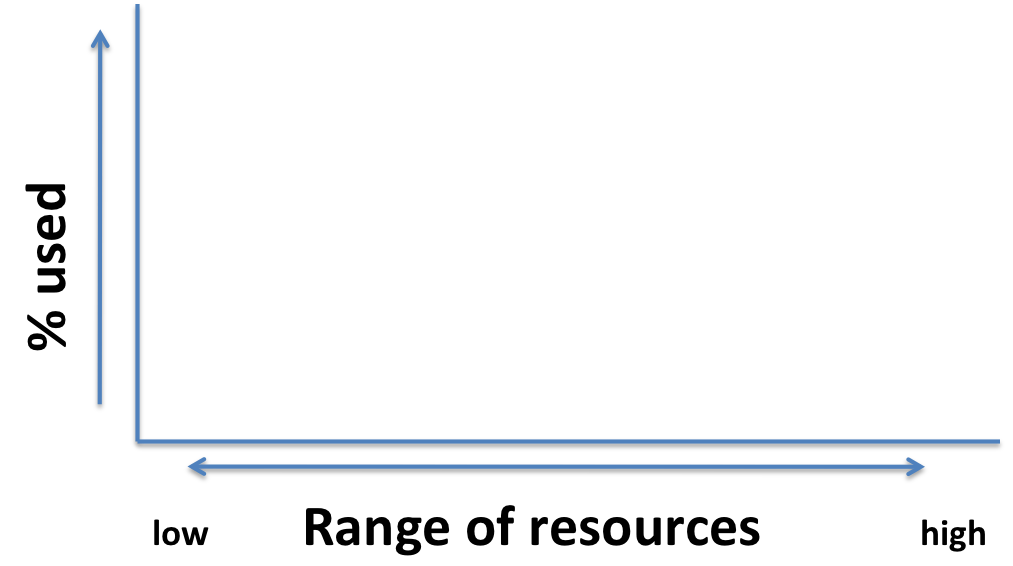
\includegraphics[height=0.67\textheight]{draw-niche.png}
        \end{center}

        \vspace{-2mm}
        Why are fundamental and realized niches different?

        \nbox{\scriptsize Fundamental niche: Total theoretical range of
            resources and environmental conditions a species can exploit.
            Realized niche: The portion of the fundamental niche that species
            actually exploits.  Interactions with other species (competitors,
            predators, parasites) can prevent a species from using full
            fundamental niche.}

    \end{adjustwidth}
\end{frame}

\subsection{Niche differentiation}

\begin{frame}[t]
    \begin{adjustwidth}{-2em}{-1.5em}
        \vspace{-3mm}
        Niche differentiation (resource partitioning):

        \nbox{\scriptsize = Evolutionary change in resource use to reduce
            fitness cost of competition between species}

        % \vspace{2mm}
        Start of competition:
        \vspace{-2mm}
        \begin{center}
        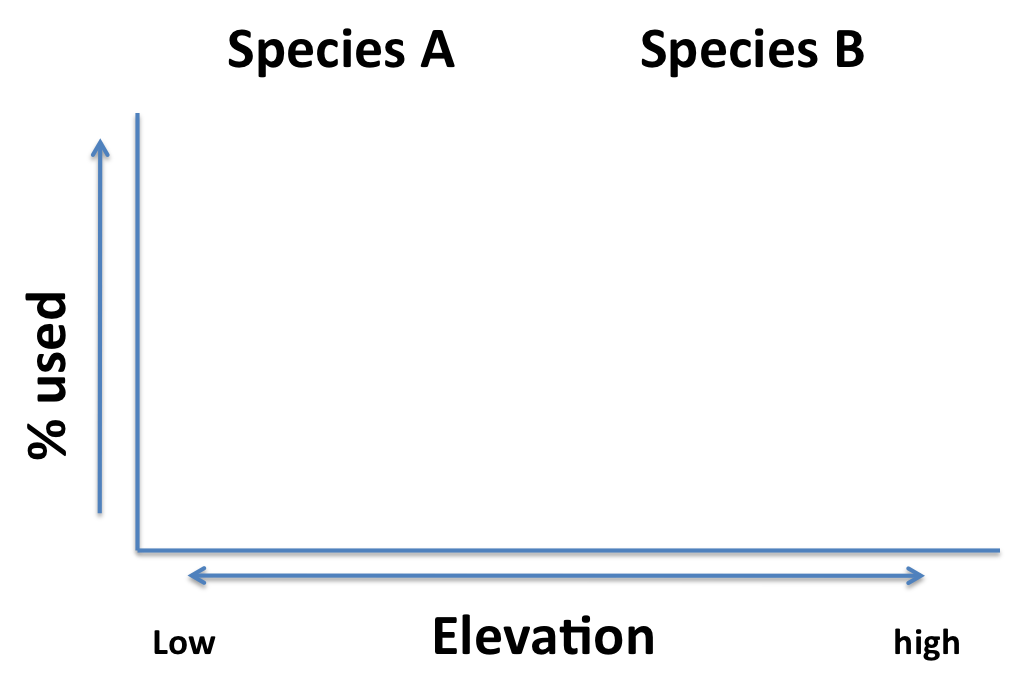
\includegraphics[height=0.75\textheight]{draw-niche-diff-elevation.png}
        \end{center}

        \nbox{Draw niches that overlap between the species.}

    \end{adjustwidth}
\end{frame}

\begin{frame}[t]
    \begin{adjustwidth}{-2em}{-1.5em}
        \vspace{-3mm}
        Niche differentiation (resource partitioning):

        \nbox{\scriptsize = Evolutionary change in resource use to reduce
            fitness cost of competition between species}

        % \vspace{2mm}
        After many generations:
        \vspace{-2mm}
        \begin{center}
        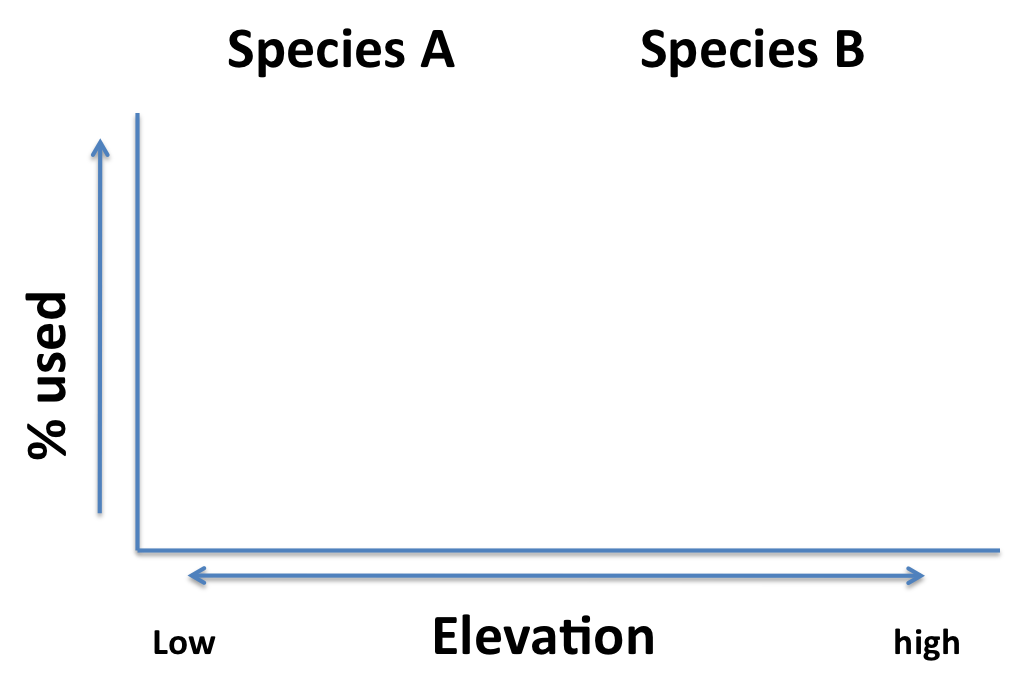
\includegraphics[height=0.65\textheight]{draw-niche-diff-elevation.png}
        \end{center}

        \vspace{-1mm}
        \nbox{\tiny Niche overlap will decrease (niches separate),
            because individuals (and their alleles) that avoid competition will
            have higher fitness}
        
        How does this relate to character displacement?

        \nbox{\scriptsize The evolutionary changes in the species traits that
            reduce competition between them}

    \end{adjustwidth}
\end{frame}


\subsection{Symmetric and asymmetric competition}

\begin{frame}[t]
    \begin{adjustwidth}{-2em}{-1.5em}
        \vspace{-3mm}
        What is symmetric and asymmetric competition?

        \vspace{2mm}
        Draw pattern predicted by symmetric competition:
        \begin{center}
        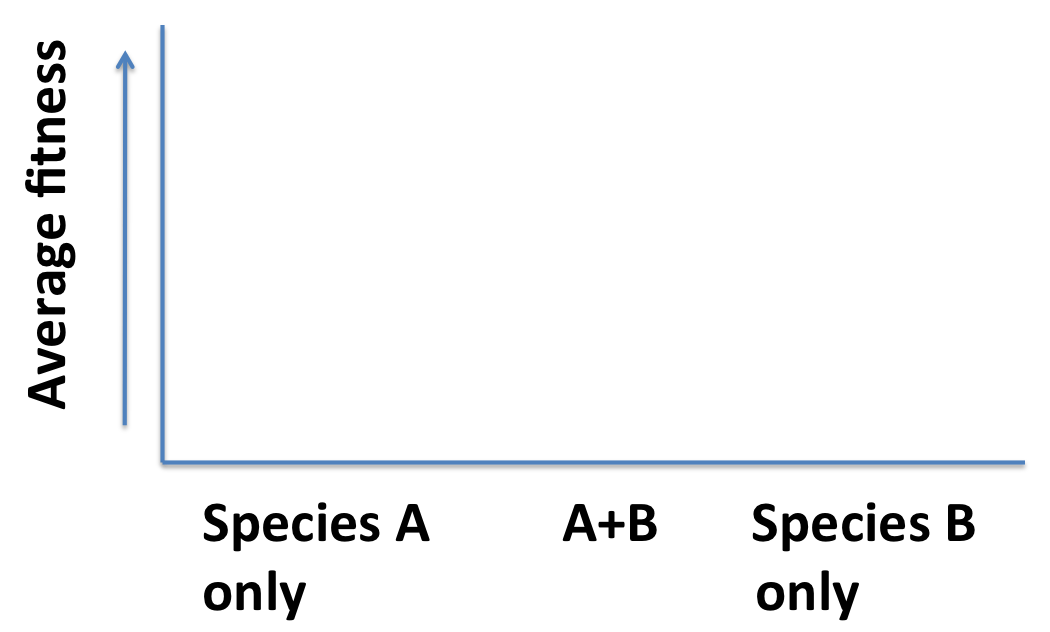
\includegraphics[height=0.65\textheight]{competition-average-fitness.png}
        \end{center}

        \nbox{\scriptsize Symmetric: Both species experience equal decrease in
            fitness due to competition.}

        \nbox{\scriptsize Asymmetric: One species experiences a greater
            decrease in fitness due to competition than the other species.}

    \end{adjustwidth}
\end{frame}

\clickerslide{
\begin{frame}[t]
    \begin{adjustwidth}{-2em}{-1.5em}
    \begin{clickerquestion}
        \item Which species will experience the most intense natural selection
            for divergence in resource use?
    \end{clickerquestion}

    \vspace{2mm}
    \begin{columns}

        \column{0.3\linewidth}

        \begin{clickeroptions}
            \item A
            \item \clickeranswer{B}
            \item A \& B equally
            \item Neither (no selection for nich divergence).
        \end{clickeroptions}

        \column{0.7\linewidth}

        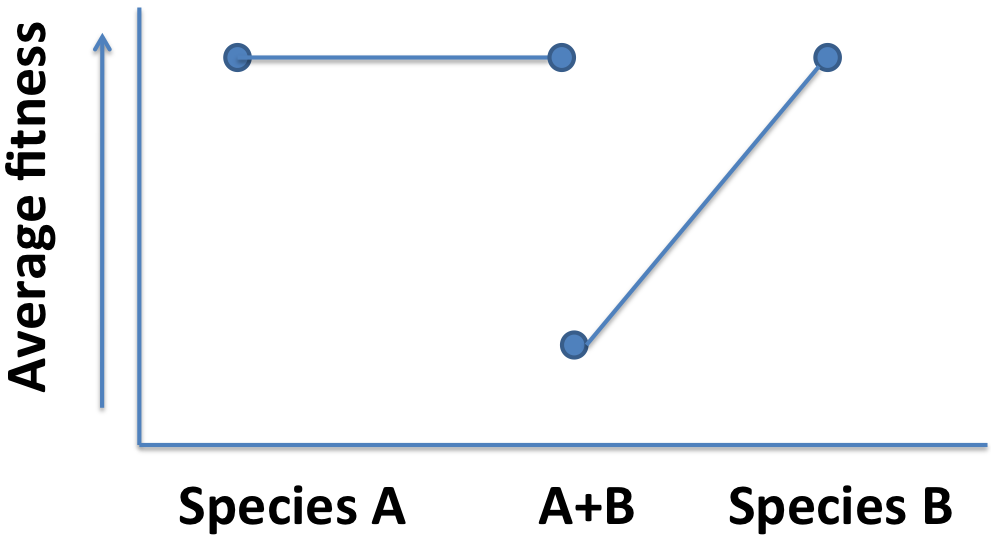
\includegraphics[width=\columnwidth]{competition-average-fitness-clicker.png}

    \end{columns}

    \end{adjustwidth}
\end{frame}
}

\subsection{Competitive exclusion}

\begin{frame}[t]
    \begin{adjustwidth}{-2em}{-1.5em}
        \vspace{-2mm}
        Competitive exclusion

        \vspace{2mm}
        E.g., G.F.\ Gause's experiments with \spp{Paramecium aurelia} and
        \spp{P.\ caudatum}

        \begin{columns}[b]

            \column{0.5\linewidth}

            \begin{figure}
                \ifhide%
                    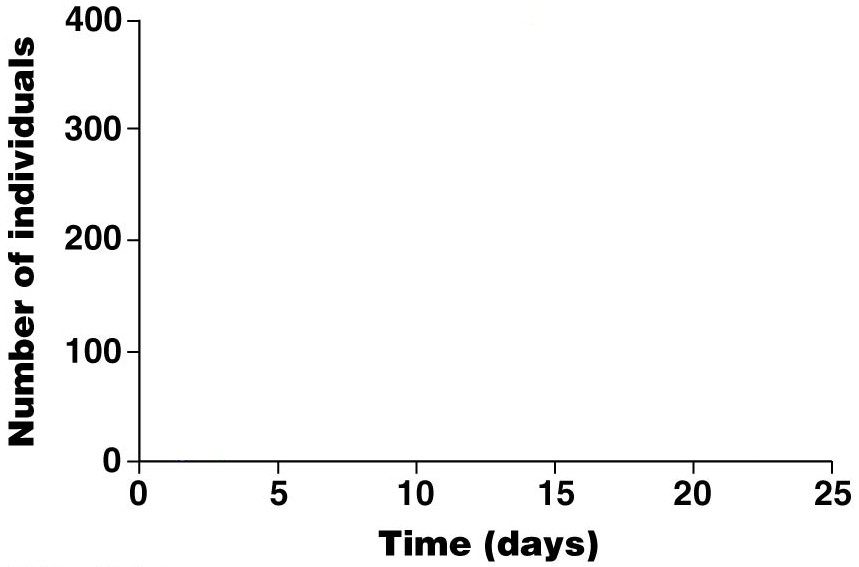
\includegraphics[width=\columnwidth]{paramecium-exclusion-blank.png}
                \else%
                    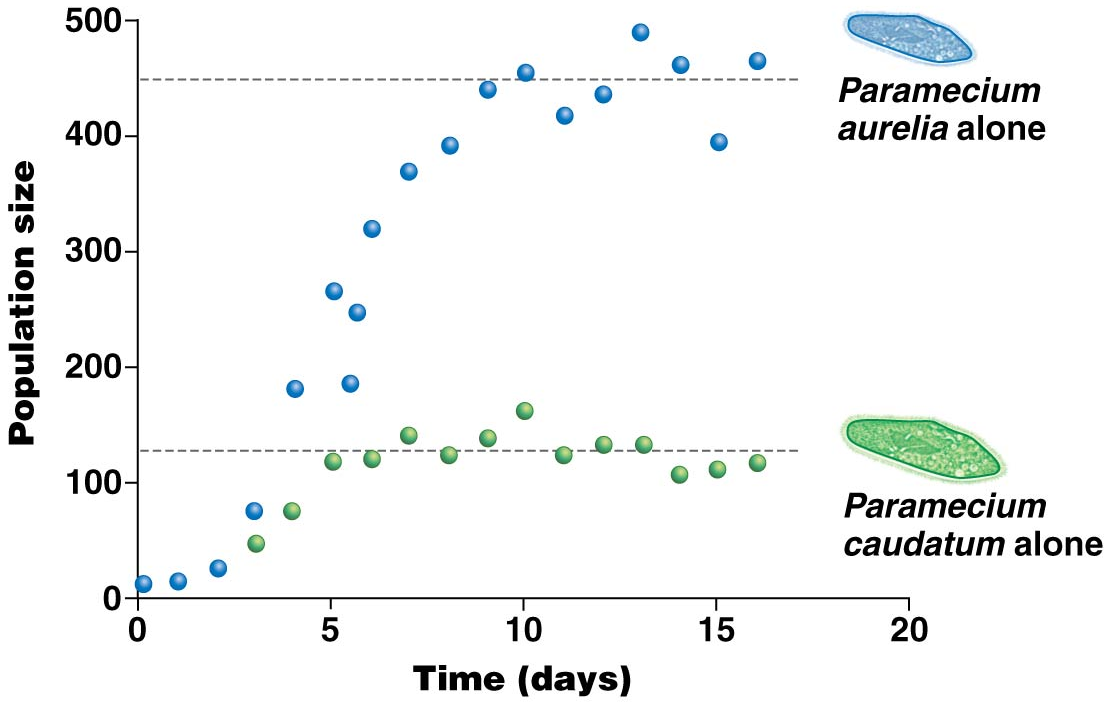
\includegraphics[width=\columnwidth]{paramecium-growth.png}
                \fi
                \caption{\Large Grown alone}
            \end{figure}

            \column{0.5\linewidth}

            \begin{figure}
                \ifhide%
                    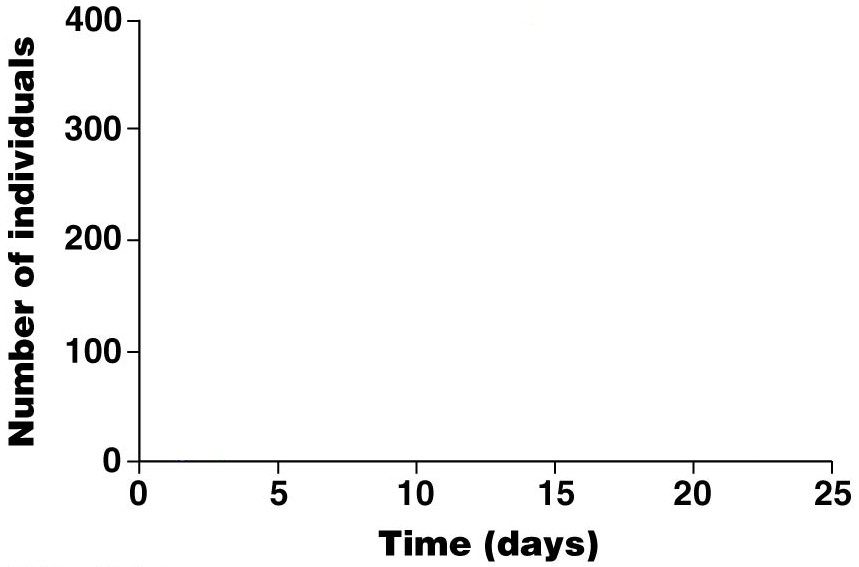
\includegraphics[width=\columnwidth]{paramecium-exclusion-blank.png}
                \else%
                    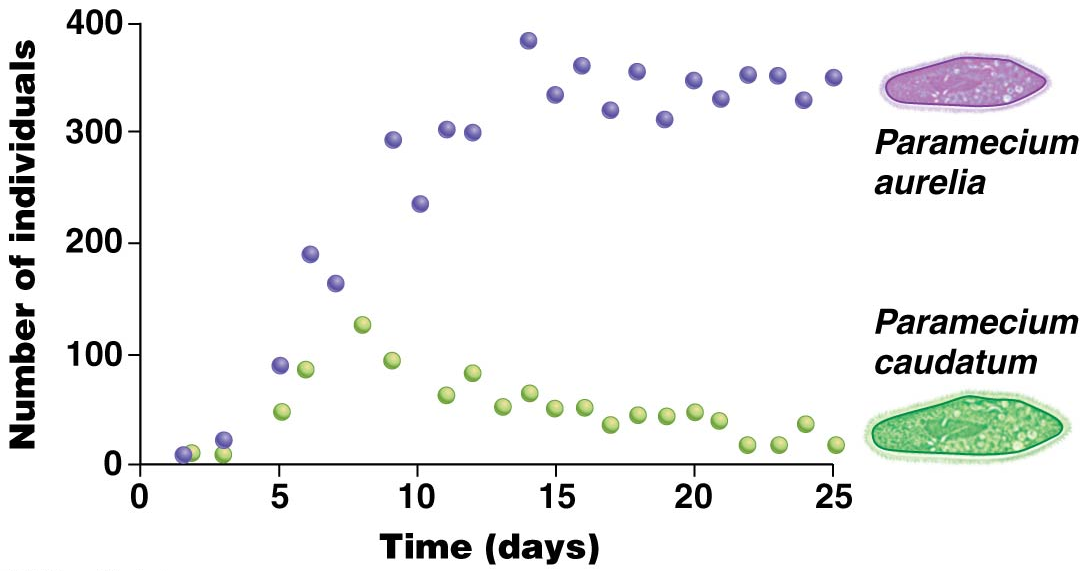
\includegraphics[width=\columnwidth]{paramecium-exclusion.png}
                \fi
                \caption{\Large Grown together}
            \end{figure}
        \end{columns}

        \nbox{When fundamental niches overlap to the extent that there's not
            enough resources outside of the overlap for either species to
            persist, one of the species will out-compete and exclude the other}
    \end{adjustwidth}
    \note[item]{So, why does \spp{P.\ caudatum} exist in nature? (Gause used
        vials) They probably occur in different places, or avoid overlap in
        other niche dimensions (e.g., water depth).}
\end{frame}

\clickerslide{
\begin{frame}
    \begin{clickerquestion}
        \item Why haven't a few plant species with the highest competitive
            ability taken over the world? (why not more competitive exclusion)
 
        \begin{clickeroptions}
            \item \clickeranswer{There are fitness trade-offs: good competitors
                    are bad at other things (e.g., colonization, drought
                    resistance, herbivore defenses).}
            \item Fundamental niche overlap is almost non-existent in nature.
            \item Most competition is symmetric.
            \item They are---species like kudzu, reed canary grass, and
                cheatgrass are taking over.
        \end{clickeroptions}
    \end{clickerquestion}
\end{frame}
}

\clickerslide{
\begin{frame}
    \begin{clickerquestion}
        \item Townsend's warblers live in the north Cascades; Hermit
            warblers live in the south Cascades. Townsend's have been moving
            steadily south, however, and out-compete Hermits. If this trend
            continues, what will be the eventual outcome? 
 
        \begin{clickeroptions}
            \item Complete niche overlap.
            \item \clickeranswer{Extinction of Hermit warblers.}
            \item Hybridization with Townsend's warblers---possibly formation
                of a new species. 
            \item Character displacement (new fundamental niche) in Townsend's
                warblers.
        \end{clickeroptions}
    \end{clickerquestion}
\end{frame}
}

\section{Observational studies of competition}

\begin{frame}[t]
    \begin{adjustwidth}{-2em}{-1.5em}
        \begin{columns}

            \column{0.45\linewidth}

            \vspace{-5mm}
            Observational studies of competition

            \vspace{2mm}
            E.g., Character displacement in Galapagos finches

            \begin{itemize}
                \item \spp{Geospiza fuliginosa} and \spp{G.\ fortis}
                    feed on similar sized seeds in allopatry

                    \vspace{2mm}
                \item What happens when they are sympatric?

                    \nbox{G.\ fortis has evolved larger bills, and there is
                        very little overlap between the species in beak size}
            \end{itemize}

            \column{0.54\linewidth}

            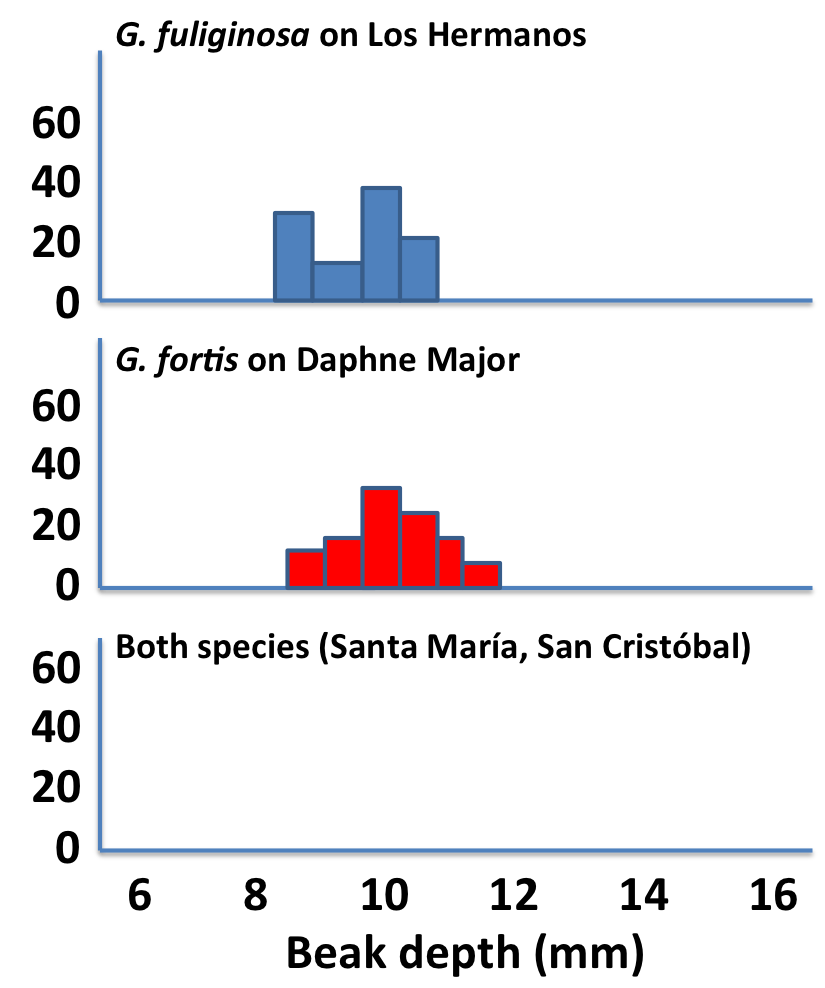
\includegraphics[width=\columnwidth]{beak-comp.png}

        \end{columns}
    \end{adjustwidth}
\end{frame}

\begin{frame}[t]
    \begin{adjustwidth}{-2em}{-1.5em}
        \begin{columns}

            \column{0.45\linewidth}

            \vspace{-5mm}
            Criticisms of observational studies

            \vspace{2mm}
            {\small
            What are other plausible hypotheses (other than competition) could
            explain this pattern?

            \nbox{\tiny \spp{G.\ fortis} is adapting to other differences
                between the islands, like food availability or predators (not
                competition with \spp{G.\ fuliginosa}).}
            \nbox{\tiny Random differences in beak size between islands
                populations (e.g., founder effect).}

            \vspace{5mm}
            How did natural experiment with \spp{G.\ magnirostris} and \spp{G.\
                fortis} on Daphne Major help?

            \nbox{\tiny Grants had long-term data on \spp{G.\ fortis} on the
                island prior to the arrival \spp{G.\ magnirostris}, and were
                able to document shift in beak size of \spp{G.\ fortis}
                population after \spp{G.\ magnirostris} arrived.}
            }

            \column{0.54\linewidth}

            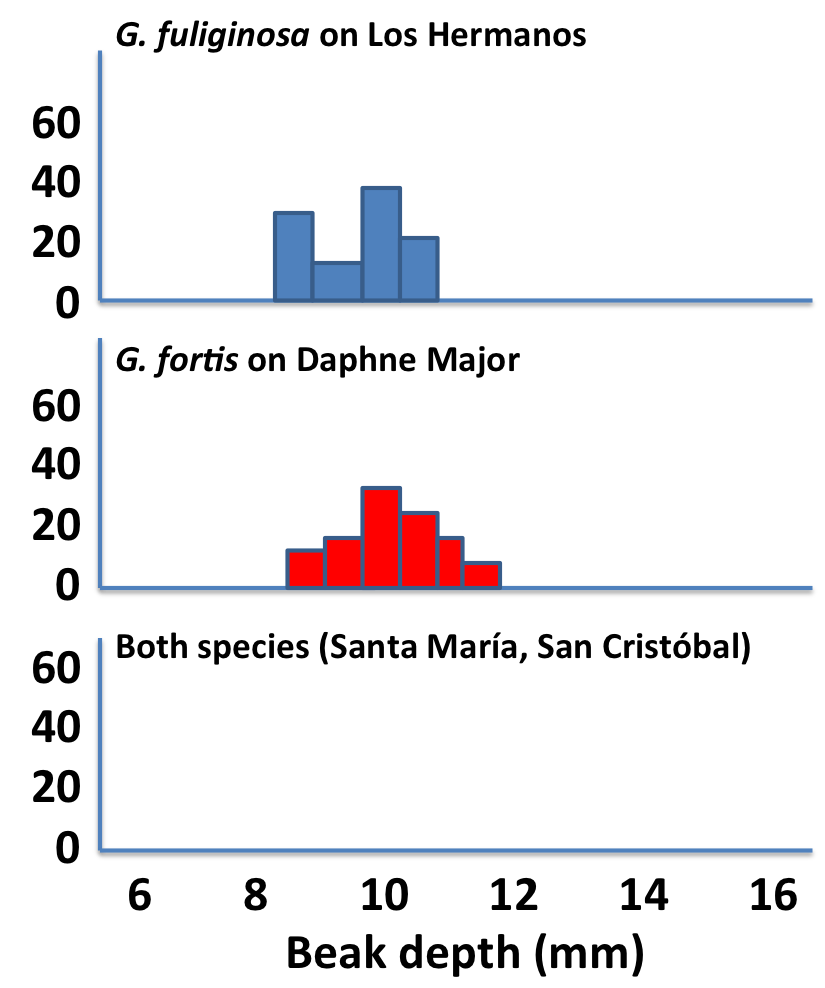
\includegraphics[width=\columnwidth]{beak-comp.png}

        \end{columns}
    \end{adjustwidth}
\end{frame}

\section{Experimental studies of competition}

\begin{frame}[t]
    \begin{adjustwidth}{-2em}{-1.5em}
        Experimental studies

        \vspace{2mm}
        E.g., Connell's study of barnacles growing in intertidal habitats

        \begin{itemize}
            \item<2-> Adults are sessile; find adult \spp{Chthamalus} in
                upper intertidal and adult \spp{Semibalanus} in lower
                intertidal.

            \item<2-> Larvae are motile; found throughout intertidal zone.

                \vspace{5mm}
            \item[$H_1$:]<3-> Adult \spp{Chthamalus} are absent from the lower
                intertidal, because \spp{Semibalanus} exclude them.

                \vspace{5mm}
            \item[$H_2$:]<3-> Adult \spp{Chthamalus} are absent from lower
                intertidal because they cannot grow there (it's outside
                their fundamental niche).
        \end{itemize}

    \end{adjustwidth}
\end{frame}

\begin{frame}[t]
    \begin{adjustwidth}{-2em}{-1.5em}
        Connell's experimental test:

        \begin{enumerate}[<+->]
            \item Take rocks from upper intertidal that are colonized by
                \spp{Chthamalus}.

                \vspace{5mm}
            \item Transfer these rocks to the lower intertidal and allow
                \spp{Semibalanus} to colonize them.

                \vspace{5mm}
            \item Divide each rock into two treatments: Remove
                \spp{Semibalanus} from one half, and leave both species on the
                other half.

                \vspace{5mm}
            \item Measure survivorship over time.
        \end{enumerate}

    \end{adjustwidth}
\end{frame}

\begin{frame}[t]
    \begin{adjustwidth}{-2em}{-1.5em}
        Questions:

        \begin{enumerate}
            \item Why did Connell split each rock into two treatments?

                \nbox{To control for variation in the composition and position
                    of the experimental rocks}

                \vspace{5mm}
            \item Would it be important to place each rock into random
                locations in the lower intertidal?

                \nbox{\scriptsize Yes---to help control for variation in
                    conditions across the lower intertidal. The variation in
                    conditions would average out across the experimental rocks
                    and would not bias the results. E.g., if he stuck all the
                    rocks in one spot, something about the conditions in that
                    spot could cause results.}

                \vspace{3mm}
            \item Why was it important for him to do many replicates (many
                rocks)?

                \nbox{To decrease the probability that the results are simply
                    due to chance or a ``weird'' rock.}
        \end{enumerate}

    \end{adjustwidth}
\end{frame}

\clickerslide{
\begin{frame}
    \begin{clickerquestion}
        \item What predictions do the two hypotheses make about the
            experimental rocks?
    \end{clickerquestion}

    \begin{adjustwidth}{-2em}{-1.5em}
    \begin{table}%[htbp]
        \centering
        \begin{tabular}{ l | L{5.2cm} | L{5.2cm} | }
            \multicolumn{1}{c}{} &
            \multicolumn{1}{c}{$H_1$ (competition)} &
            \multicolumn{1}{c}{$H_2$ (fundamental niche)} \\
            \cline{2-3}
            \textcolor{red}{1)} &
            \spp{Chthamalus} has low survival in presence of \spp{Semibalanus} &
            \spp{Chthamalus} grows better than \spp{Semibalanus} \\
            \cline{2-3}
            \textcolor{red}{2)} &
            \spp{Semibalanus} only grows when \spp{Chthamalus} is present &
            \spp{Semibalanus} grows better than \spp{Chthamalus} \\
            \cline{2-3}
            \textcolor{red}{3)} &
            \spp{Chthamalus} has low survival in presence of \spp{Semibalanus} &
            \spp{Semibalanus} has low survival in presence or absence of \spp{Chthamalus} \\
            \cline{2-3}
            \textcolor{red}{4)} &
            \clickeranswer{\spp{Chthamalus} has low survival in presence of
                \spp{Semibalanus}} &
            \clickeranswer{\spp{Chthamalus} has low survival in presence or absence
                \spp{Semibalanus}} \\
            \cline{2-3}
        \end{tabular}
    \end{table}
    \end{adjustwidth}
\end{frame}
}

\clickerslide{
\begin{frame}
    \begin{clickerquestion}
        \item How would you test the hypothesis that \spp{Semibalanus} can't
            grow in the upper intertidal (outside of its fundamental niche)? 

        \begin{clickeroptions}
            \item Survey all of the appropriate habitats---if \spp{Semibalanus}
                is never found in the upper intertidal, it can't grow there.
            \item \clickeranswer{Move rocks containing \spp{Semibalanus} to the
                    upper intertidal and monitor survival in presence/absence
                    of \spp{Chthamalus}.} 
            \item Document the physical conditions (hours exposed to air,
                average temperature, etc.) in the upper versus lower
                intertidal. 
            \item No additional work is necessary---you already know they can't
                (larvae are found there). 
        \end{clickeroptions}
    \end{clickerquestion}
\end{frame}
}

\end{document}

\clickerslide{
\begin{frame}
    \begin{clickerquestion}
        \item 
        \begin{clickeroptions}
            \item 
            \item 
            \item 
            \item 
        \end{clickeroptions}
    \end{clickerquestion}
\end{frame}
}

\clickerpost{
{
\usebackgroundtemplate{\includegraphics[page=17,width=\paperwidth]{./24-Radiation-extinction.pdf}}
\begin{frame}[t,plain]
    \begin{adjustwidth}{-2em}{-1.5em}
        \cmask{Answer: 3}
    \end{adjustwidth}
\end{frame}
}
}

